\section{Fondamenti}

\begin{softnote}
	Questa sezione introduce i concetti fondamentali necessari per comprendere il resto del corso. Non preoccuparti se all'inizio alcune definizioni sembrano astratte: diventeranno chiare con gli esempi concreti nelle sezioni successive.
\end{softnote}

\subsection{Introduzione al corso}

\subsubsection{Requisiti}
\begin{itemize}
	\item Fondamenti di matematica discreta e grafi
	\item Calcolo delle probabilità
	\item Basi di C $\to$ si studia Java (Classi e Oggetti)\footnote{Java è il male}
	\item Le procedure ricorsive sono come l'Ave Maria (STUDIA: c'è nell'esame)
\end{itemize}

\begin{nota}
	La ricorsione è \textbf{fondamentale} in questo corso. Se non ti senti sicuro, ripassa prima di procedere: fibonacci, fattoriale, e i concetti base di chiamate ricorsive.
\end{nota}

\subsubsection{Programma del corso}
\begin{itemize}
	\item Divide et Impera
	\item Programmazione dinamica
	\item Algoritmi Greedy
	\item Grafi $\to$ Nodi e archi
\end{itemize}

\begin{softnote}
	Questi quattro argomenti sono le \textbf{tecniche algoritmiche} principali. Ogni tecnica è un "modo di pensare" per risolvere problemi complessi:
	\begin{itemize}
		\item \textbf{Divide et Impera}: spezza il problema in pezzi piccoli
		\item \textbf{Programmazione Dinamica}: memorizza soluzioni parziali per evitare ricalcoli
		\item \textbf{Greedy}: fai sempre la scelta localmente migliore
		\item \textbf{Grafi}: rappresenta problemi come reti di connessioni
	\end{itemize}
\end{softnote}

\subsubsection{Struttura del modulo}
48 ore di lezione: 4 ore a settimana + 9 ore di studio personale.\footnote{Sì, lo so, è una noia, ma serve.}
Non usare ChatGPT o altri strumenti simili.

I lucidi non bastano (purtroppo).

Se proprio devi, usa \textbf{Anthropic CLAUDE}.

\subsubsection{Modalità di esame}
\begin{itemize}
	\item \textbf{Prima parte:} 15 domande a risposta multipla
	(almeno 4 su codice Java -- CODE RUNNER)
	\item \textbf{Seconda parte:} Progettare una soluzione algoritmica
	\item \textbf{Se va male:} Può fare orale se ha dubbi (Ave o Maria\dots)
\end{itemize}

% ================================================================
\subsection{Il ruolo degli algoritmi nell'informatica}

\begin{softnote}
	Prima di tuffarci nei dettagli tecnici, capiamo \textbf{perché} gli algoritmi sono importanti. Un algoritmo è semplicemente una "ricetta" per risolvere un problema al computer.
\end{softnote}

\subsubsection{Cos'è un algoritmo?}

\begin{definizione}[Algoritmo]
	Procedura di calcolo ben definita: dato un input (anche nullo), produce un output
	in tempo finito.
\end{definizione}

\begin{nota}
	\textbf{In parole semplici:} un algoritmo è una sequenza di passi precisi che trasforma dei dati di partenza (input) in un risultato (output). Deve sempre finire in tempo ragionevole.
	
	\textbf{Esempio quotidiano:} una ricetta di cucina è un algoritmo:
	\begin{itemize}
		\item \textbf{Input}: ingredienti (farina, uova, zucchero)
		\item \textbf{Passi}: mescola, cuoci a 180°C per 30 minuti
		\item \textbf{Output}: torta
	\end{itemize}
\end{nota}

\begin{definizione}[Problema computazionale]
	Relazione input/output desiderata. L'algoritmo specifica \textit{come} ottenerla.
\end{definizione}

\begin{softnote}
	\textbf{Differenza chiave:}
	\begin{itemize}
		\item \textbf{Problema}: ``Voglio ordinare una lista di numeri'' (COSA)
		\item \textbf{Algoritmo}: ``Confronta elementi a coppie e scambiali se necessario'' (COME)
	\end{itemize}
	Il problema dice \textit{cosa} vogliamo ottenere, l'algoritmo dice \textit{come} farlo.
\end{softnote}

\begin{definizione}[Algoritmo corretto]
	Termina producendo il risultato corretto per ogni istanza valida.
\end{definizione}

\begin{osservazione}
	Non sempre esiste un algoritmo: il problema della fermata è indecidibile.
\end{osservazione}

\begin{nota}
	\textbf{Cosa significa ``indecidibile''?} Esistono problemi per cui è matematicamente impossibile scrivere un algoritmo generale che funzioni sempre. Il famoso ``problema della fermata'' chiede: ``Dato un programma qualsiasi, terminerà mai?'' È stato dimostrato che non esiste un algoritmo che possa rispondere a questa domanda per tutti i programmi possibili.
\end{nota}


\subsection{Esempio di algoritmo ricorsivo}

\begin{softnote}
	Ora vediamo un esempio concreto: calcolare i numeri di Fibonacci. Questo ci permetterà di capire la differenza tra un algoritmo \textbf{corretto} (che funziona) e uno \textbf{efficiente} (che funziona velocemente).
\end{softnote}

\begin{nota}
	\textbf{Cosa sono i numeri di Fibonacci?}
	
	È una sequenza di numeri dove ogni numero è la somma dei due precedenti:
	\[
	0, 1, 1, 2, 3, 5, 8, 13, 21, 34, \ldots
	\]
	
	Definizione formale:
	\[
	F_0 = 0, \quad F_1 = 1, \quad F_n = F_{n-1} + F_{n-2} \text{ per } n \geq 2
	\]
	
	\textbf{Esempio:} $F_5 = F_4 + F_3 = 3 + 2 = 5$
\end{nota}

\begin{nota}
	Le convenzioni usate per il pseudocodice sono a pag. 19 del [CLRS].
\end{nota}

\begin{algorithm}[H]
	\caption{FibonacciR}
	\KwIn{$n \geq 0$}
	\KwOut{$F_n$}
	\If{$n = 0$}{\Return $0$\;}
	\If{$n = 1$}{\Return $1$\;}
	\Return FibonacciR($n-1$) + FibonacciR($n-2$)\;
\end{algorithm}

\begin{softnote}
	\textbf{Come funziona questo algoritmo?}
	
	Traduce direttamente la definizione matematica in codice:
	\begin{enumerate}
		\item Se $n=0$ restituisci 0 (caso base)
		\item Se $n=1$ restituisci 1 (caso base)
		\item Altrimenti, calcola $F_{n-1}$ e $F_{n-2}$ ricorsivamente e sommali
	\end{enumerate}
	
	\textbf{Esempio per $n=4$:}
	\begin{itemize}
		\item Calcola $F_3 + F_2$
		\item $F_3 = F_2 + F_1$, quindi serve calcolare $F_2$ due volte!
		\item $F_2 = F_1 + F_0 = 1 + 0 = 1$
		\item Risultato finale: $F_4 = 3$
	\end{itemize}
\end{softnote}

L'algoritmo è corretto? \textbf{Sì!}

Per ogni input valido, termina? \textbf{Sì, assumendo che input sia sempre un intero n  $\geq$ 0}

Se sì, calcola il valore giusto? \textbf{Sì, perché l'algoritmo codifica la definizione ricorsiva.}

Quanto \textbf{tempo} richiede per terminare?

\begin{figure}[H]
	\centering
	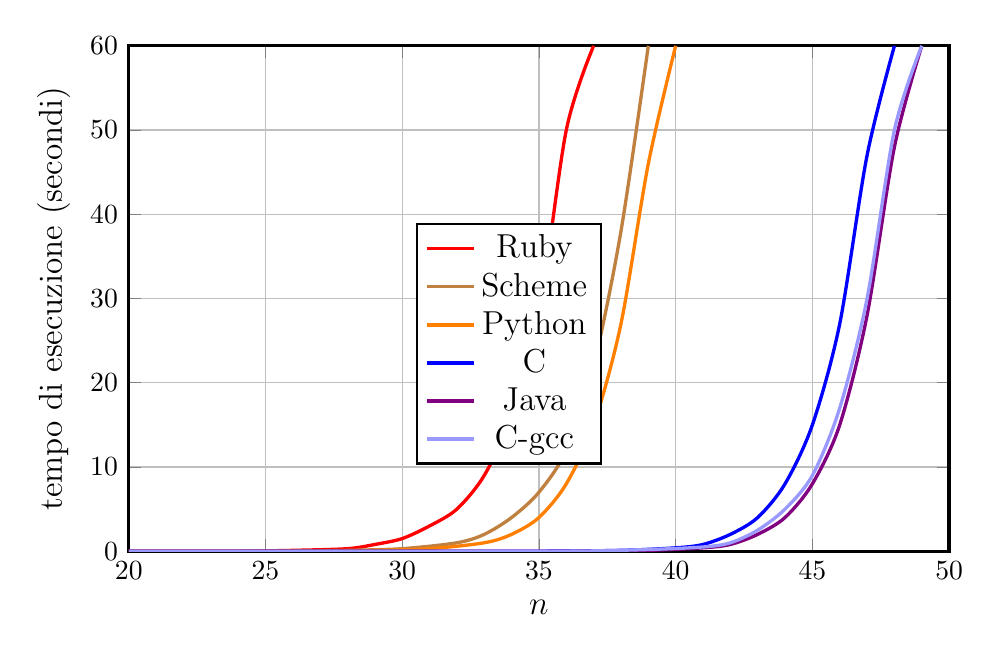
\begin{tikzpicture}
		\begin{axis}[
			xlabel={$n$},
			ylabel={tempo di esecuzione (secondi)},
			xmin=20, xmax=50,
			ymin=0, ymax=60,
			grid=major,
			width=12cm,
			height=8cm,
			legend style={
				at={(0.35,0.65)},
				anchor=north west,
				font=\large,
				fill=white,
				draw=black,
				line width=0.8pt
			},
			tick label style={font=\normalsize},
			label style={font=\large},
			line width=1.2pt
			]
			
			% Ruby
			\addplot[red, very thick, smooth] coordinates {
				(20,0) (22,0) (24,0) (26,0.1) (28,0.3) (29,0.8) (30,1.5)
				(31,3) (32,5) (33,9) (34,16) (35,28) (36,50) (37,60)
			};
			\addlegendentry{Ruby}
			
			% Scheme
			\addplot[brown, very thick, smooth] coordinates {
				(20,0) (23,0) (26,0) (28,0.1) (30,0.3) (32,1) (33,2)
				(34,4) (35,7) (36,12) (37,22) (38,38) (39,60)
			};
			\addlegendentry{Scheme}
			
			% Python
			\addplot[orange, very thick, smooth] coordinates {
				(20,0) (24,0) (27,0) (29,0.1) (31,0.3) (33,1) (34,2)
				(35,4) (36,8) (37,15) (38,27) (39,46) (40,60)
			};
			\addlegendentry{Python}
			
			% C
			\addplot[blue, very thick, smooth] coordinates {
				(20,0) (30,0) (35,0) (38,0.1) (40,0.4) (41,0.8) (42,2)
				(43,4) (44,8) (45,15) (46,27) (47,47) (48,60)
			};
			\addlegendentry{C}
			
			% Java
			\addplot[violet, very thick, smooth] coordinates {
				(20,0) (30,0) (36,0) (39,0.1) (41,0.4) (42,0.8) (43,2)
				(44,4) (45,8) (46,15) (47,28) (48,48) (49,60)
			};
			\addlegendentry{Java}
			
			% C-gcc
			\addplot[blue!40, very thick, smooth] coordinates {
				(20,0) (30,0) (36,0) (39,0.2) (41,0.5) (42,1) (43,2.5)
				(44,5) (45,9) (46,17) (47,30) (48,50) (49,60)
			};
			\addlegendentry{C-gcc}
			
		\end{axis}
	\end{tikzpicture}
	\caption{Confronto dei tempi di esecuzione dell'algoritmo ricorsivo \texttt{FibonacciR} in diversi linguaggi. I linguaggi interpretati (Ruby, Scheme, Python) saturano a valori di $n$ molto più bassi rispetto ai linguaggi compilati (C, Java, C-gcc).}
	\label{fig:fibonacci-linguaggi}
\end{figure}


\begin{hardnote}
	\textbf{Problema grave:} anche se l'algoritmo è corretto, è \textbf{terribilmente lento}.
	
	Per $n=50$ impiega diversi minuti, mentre un algoritmo migliore lo calcola istantaneamente. Il problema è che ricalcola gli stessi valori moltissime volte.
\end{hardnote}

\newpage
\subsubsection*{Calcolo della complessità computazionale}

\begin{softnote}
	La \textbf{complessità} misura quanto ``costa'' eseguire un algoritmo. Non misuriamo i secondi (dipendono dal computer), ma il numero di operazioni in funzione della dimensione dell'input.
\end{softnote}

\begin{definizione}[Efficienza]
	Risorse (tempo e spazio) richieste in funzione della dimensione $n$ dell'input.
\end{definizione}

\begin{definizione}[Algoritmo vs.\ Implementazione]
	L'algoritmo è un concetto \textbf{astratto} ($\neq$ implementazione):
	descrive \textit{come} risolvere un problema indipendentemente dal linguaggio.
	L'implementazione è un \textbf{programma concreto}, ovvero la traduzione
	dell'algoritmo in un linguaggio comprensibile dalla macchina.
\end{definizione}

\begin{nota}
	\textbf{Analogia:}
	\begin{itemize}
		\item \textbf{Algoritmo} = ricetta scritta in italiano (``mescola gli ingredienti'')
		\item \textbf{Implementazione} = ricetta tradotta in giapponese per un cuoco giapponese
	\end{itemize}
	L'idea (algoritmo) è la stessa, cambia solo la forma (implementazione).
\end{nota}

\begin{nozione}[Algoritmo efficiente]
	Andiamo a cercare l'algoritmo efficiente:
	\begin{itemize}
		\item \textbf{Efficiente:} usa poche risorse
		\item \textbf{Risorse:} tempo e spazio richiesti dall'algoritmo
		per produrre l'output
	\end{itemize}
\end{nozione}

\begin{teorema}[Algoritmo vs.\ hardware]
	Con $n = 10^7$ interi da ordinare:
	\begin{align*}
		t_A &= \frac{2(10^7)^2}{10^{10}} \approx 5.5\ \text{ore}
		\quad\text{(InsSort, } 10^9 \text{ istr/s)} \\
		t_B &= \frac{50 \cdot 10^7 \log_2 10^7}{10^6} \approx 20\ \text{min}
		\quad\text{(MergeSort, } 10^6 \text{ istr/s)}
	\end{align*}
	L'algoritmo migliore batte l'hardware più veloce.
\end{teorema}

\begin{hardnote}
	\textbf{Lezione fondamentale:} un algoritmo efficiente su un computer lento batte un algoritmo inefficiente su un computer veloce.
	
	Nell'esempio:
	\begin{itemize}
		\item Computer A: 10× più veloce, ma usa InsertionSort (algoritmo lento)
		\item Computer B: 10× più lento, ma usa MergeSort (algoritmo veloce)
	\end{itemize}
	Risultato: B finisce in 20 minuti, A impiega 5.5 ore!
\end{hardnote}

\textbf{Possiamo fare meglio?}

\subsubsection*{Ottimizzazione: FibonacciI }
\begin{algorithm}[H]
	\caption{FibonacciI}
	\KwIn{Intero positivo $n$}
	\KwOut{Il valore $F_n$}
	\If{$n = 0$}{\Return $0$\;}
	\If{$n = 1$}{\Return $1$\;}
	$\mathit{pprev} = 0$\;
	$\mathit{prev} = 1$\;
	\For{$i = 2$ \KwTo $n$}{
		$f = \mathit{prev} + \mathit{pprev}$\;
		$\mathit{pprev} = \mathit{prev}$\;
		$\mathit{prev} = f$\;
	}
	\Return $f$\;
\end{algorithm}

\begin{softnote}
	\textbf{Come funziona FibonacciI (iterativo)?}
	
	Invece di chiamare ricorsivamente la funzione, mantiene in memoria solo gli ultimi due valori e li aggiorna ad ogni passo:
	
	\begin{itemize}
		\item Inizia con $F_0=0$ e $F_1=1$
		\item Calcola $F_2 = F_1 + F_0 = 1$
		\item Calcola $F_3 = F_2 + F_1 = 2$
		\item Calcola $F_4 = F_3 + F_2 = 3$
		\item E così via fino a $F_n$
	\end{itemize}
	
	\textbf{Vantaggio:} ogni numero viene calcolato \textbf{una sola volta}, non milioni di volte come nella versione ricorsiva!
\end{softnote}

La complessità è:
\[
T(0) = 2, \quad T(1) = 3, \quad T(n) = 4 + 2n + 4(n-1) + 1 = 6n + 1
\]

La crescita è \textbf{lineare in $n$}.


\begin{center}
	\begin{tabular}{lll}
		\toprule
		Algoritmo & Complessità & $n=50$ \\
		\midrule
		Ricorsivo & $(1.4)^n$   & minuti \\
		Iterativo & $\Theta(n)$ & istantaneo \\
		\bottomrule
	\end{tabular}
\end{center}

\begin{hardnote}
	\textbf{Confronto drammatico:}
	\begin{itemize}
		\item FibonacciR (ricorsivo): per $n=50$ fa circa $2^{25} \approx 33$ milioni di chiamate $\to$ minuti
		\item FibonacciI (iterativo): per $n=50$ fa esattamente 50 iterazioni $\to$ istantaneo
	\end{itemize}
	
	Questo dimostra che due algoritmi che risolvono lo stesso problema possono avere prestazioni \textbf{radicalmente diverse}.
\end{hardnote}

\noindent\textbf{Modello RAM:} ogni operazione elementare ha costo $1$;
parola di memoria a dimensione fissa.

\begin{nota}
	Il \textbf{modello RAM} (Random Access Machine) è una semplificazione che assumiamo per analizzare gli algoritmi:
	\begin{itemize}
		\item Ogni operazione base (somma, confronto, assegnazione) costa 1
		\item La memoria è infinita e accedervi costa 1
		\item Un solo processore esegue un'istruzione alla volta
	\end{itemize}
	
	Non è realistico (nella realtà ci sono cache, processori multipli, ecc.), ma è utile per confrontare algoritmi in modo uniforme.
\end{nota}

\subsection{Esempi di problemi computazionali da risolvere in aula}

\begin{softnote}
	Ora vediamo alcuni problemi classici che ti aiuteranno a capire come si progettano e analizzano gli algoritmi. Studia bene questi esempi: sono fondamentali per l'esame!
\end{softnote}

\subsubsection*{Indici dei due numeri che sommati danno N}
\textbf{Problema:} Data una matrice di interi \texttt{nums} e un intero \texttt{target}, restituisci gli indici dei due numeri tali che la loro somma sia uguale a \texttt{target}. Puoi assumere che ogni input abbia esattamente una soluzione, e non puoi usare lo stesso elemento due volte. Puoi restituire la risposta in qualsiasi ordine.

\begin{nota}
	\textbf{In parole semplici:} hai un array di numeri e un numero obiettivo. Devi trovare due numeri nell'array che sommati danno il numero obiettivo, e restituire le loro posizioni.
	
	\textbf{Esempio:}
	\begin{itemize}
		\item Input: \texttt{nums = [2, 7, 11, 15]}, \texttt{target = 9}
		\item Output: \texttt{[0, 1]}
		\item Spiegazione: \texttt{nums[0] + nums[1] = 2 + 7 = 9}
	\end{itemize}
\end{nota}

\begin{algorithm}[H]
	\caption{twoSum (Brute Force)}
	\KwIn{\texttt{nums[0\ldots n-1]}, \texttt{target}}
	\KwOut{\{i, j\} tali che \texttt{nums[i] + nums[j] = target}, $i \neq j$}
	\For{$i = 0$ \KwTo $n-2$}{
		\For{$j = i+1$ \KwTo $n-1$}{
			\If{\texttt{nums[i] + nums[j] == target}}{
				\KwRet $\{i, j\}$\;
			}
		}
	}
\end{algorithm}

\begin{softnote}
	\textbf{Come funziona l'algoritmo?}
	
	Prova tutte le possibili coppie di numeri:
	\begin{enumerate}
		\item Fisso il primo numero (indice $i$)
		\item Controllo tutti i numeri successivi (indice $j > i$)
		\item Se $nums[i] + nums[j] = target$, ho trovato la coppia!
	\end{enumerate}
	
	Si chiama ``brute force'' (forza bruta) perché prova semplicemente tutte le combinazioni possibili.
\end{softnote}

\noindent\textbf{Invariante:} Dopo ogni iterazione esterna, tutti gli elementi da $0$ a $i-1$ sono stati confrontati con tutti gli elementi successivi.

\begin{nota}
	L'\textbf{invariante di ciclo} è una proprietà che rimane vera ad ogni iterazione. Serve per dimostrare che l'algoritmo è corretto. In questo caso: ``alla fine dell'iterazione $i$, abbiamo controllato tutte le coppie che iniziano con indici da $0$ a $i$.''
\end{nota}

\noindent\textbf{Complessità:}
\begin{itemize}
	\item Caso migliore: $\Theta(1)$ (se la coppia è trovata subito)
	\item Caso peggiore: $\Theta(n^2)$
\end{itemize}

\noindent\textbf{Calcolo della complessità temporale (caso peggiore):}

L'algoritmo esegue due cicli annidati. Il ciclo esterno itera $n-1$ volte, e per ogni $i$ il ciclo interno itera $n-1-i$ volte. Quindi:

\[
T(n) = \sum_{i=0}^{n-2} (n-1-i) = \sum_{k=1}^{n-1} k = 	\frac{(n-1)n}{2} \in \Theta(n^2)
\]

\begin{softnote}
	\textbf{Perché $\Theta(n^2)$?}
	
	Il ciclo esterno fa $n$ passi, e per ognuno il ciclo interno fa in media $n/2$ passi. In totale: $n \times n/2 = n^2/2$ operazioni. Siccome ignoriamo le costanti, rimane $n^2$.
	
	\textbf{Esempio concreto:} con $n=100$ elementi, l'algoritmo fa circa $100 \times 100 / 2 = 5000$ confronti.
\end{softnote}

La complessità spaziale è $\Theta(1)$, poiché usiamo solo variabili costanti. 

\subsubsection*{Codice JAVA}
\begin{lstlisting}[language=Java, numbers=none, basicstyle=\ttfamily\footnotesize]
	class twoSum {
		public int[] twoSum(int[] nums, int target) {
			for (int i = 0; i < nums.length; i++) {
				for (int j = i + 1; j < nums.length; j++) {
					if (nums[i] + nums[j] == target) {
						return new int[]{i, j};
					}
				}
			}
			return new int[]{};  // nessuna soluzione trovata
		}
	}
\end{lstlisting}

\begin{nota}
	\textbf{Nota sul codice Java:}
	\begin{itemize}
		\item \texttt{nums.length} restituisce la lunghezza dell'array
		\item \texttt{new int[]\{i, j\}} crea un nuovo array con due elementi
		\item Il \texttt{return} interrompe immediatamente l'esecuzione quando trova la soluzione
	\end{itemize}
\end{nota}

\subsubsection*{Problema dell'inversione numerica}

\begin{softnote}
	Questo problema insegna a manipolare le cifre di un numero usando aritmetica modulare. È un classico per imparare operazioni su interi.
\end{softnote}

\begin{algorithm}[H]
	\caption{Inversione numerica}
	\label{alg:inversione}
	
	\KwIn{Intero $x$ rappresentato con segno a 32 bit}
	\KwOut{Intero $y$ con le cifre di $x$ invertite}
	
	$y = 0$\tcp*{Inizializza risultato}
	$sign = 1$\tcp*{Memorizza segno}
	
	$sign = (x < 0) ? -1 : 1$\tcp*{Memorizza segno di x}
	$x = |x|$\tcp*{Rende x positivo}
	
	\While{$x > 0$}{
		$digit = x \bmod 10$\tcp*{Estrae ultima cifra}
		$y = y \times 10 + digit$\tcp*{Aggiunge a y}
		$x = \lfloor x / 10 \rfloor$\tcp*{Rimuove cifra}
	}
	
	\Return{$y \times sign$}\tcp*{Restituisce con segno}
\end{algorithm}

\begin{softnote}
	\textbf{Come funziona l'inversione?}
	
	\textbf{Esempio:} inverti 1234
	\begin{enumerate}
		\item $digit = 1234 \bmod 10 = 4$, $y = 0 \times 10 + 4 = 4$, $x = 123$
		\item $digit = 123 \bmod 10 = 3$, $y = 4 \times 10 + 3 = 43$, $x = 12$
		\item $digit = 12 \bmod 10 = 2$, $y = 43 \times 10 + 2 = 432$, $x = 1$
		\item $digit = 1 \bmod 10 = 1$, $y = 432 \times 10 + 1 = 4321$, $x = 0$
	\end{enumerate}
	
	\textbf{Trucchi usati:}
	\begin{itemize}
		\item $n \bmod 10$ estrae l'ultima cifra
		\item $\lfloor n / 10 \rfloor$ rimuove l'ultima cifra
		\item Moltiplicare per 10 e sommare ``costruisce'' il numero invertito
	\end{itemize}
\end{softnote}

\textbf{Complessità.}
Sia $k$ il numero di cifre decimali di $|x|$. Allora
\[
T(k) =
\begin{cases}
	6       & \text{se } x = 0,\\
	5k + 6  & \text{se } x > 0,\\
	5k + 8  & \text{se } x < 0,
\end{cases}
\qquad\Rightarrow\qquad
T(k) = \mathcal{O}(k).
\]

\begin{center}
	La complessità dell'algoritmo è lineare nel numero di cifre.
\end{center}

\begin{nota}
	Se il numero ha $k$ cifre, il ciclo while viene eseguito esattamente $k$ volte (una per ogni cifra). Quindi la complessità è $O(k)$, dove $k = \log_{10}(n)$ per un numero $n$.
	
	\textbf{Esempio:} il numero 12345 ha 5 cifre, quindi $k=5$ e il ciclo fa 5 iterazioni.
\end{nota}


\begin{nota}
	L'\textbf{operatore ternario} è definito come:
	
	\texttt{x = (espressione booleana) ? v1 : v2}
	
	\begin{itemize}
		\item se l'espressione booleana è vera viene usata \texttt{v1}
		\item se l'espressione booleana è falsa viene usata \texttt{v2}
	\end{itemize}
	
	\textbf{Esempio:} \texttt{max = (a > b) ? a : b} assegna a \texttt{max} il valore più grande tra \texttt{a} e \texttt{b}.
\end{nota}

\subsubsection*{Container con più acqua}

\begin{softnote}
	Questo è un problema di ottimizzazione: dobbiamo trovare il rettangolo di area massima. Introduciamo la tecnica dei ``due puntatori'' che è molto utile per problemi su array.
\end{softnote}

Si consideri un array di interi non negativi $height$ di lunghezza $n$.
Per ogni $i$, la retta verticale ha estremi $(i,0)$ e $(i,height[i])$.
Si vogliono trovare due rette che, insieme all'asse $x$, formino un
contenitore che possa contenere la massima quantità d'acqua.

\medskip
Nel nostro esempio poniamo
\[
A = [4,6,3,5].
\]

L'area del contenitore formato dalle rette in posizione $i$ e $j$
($i < j$) è data da
\[
\mathrm{area}(i,j) = (j-i)\,\min(A[i],A[j]).
\]

\begin{nota}
	\textbf{Perché questa formula?}
	
	L'area di un rettangolo è: $\text{base} \times \text{altezza}$
	\begin{itemize}
		\item \textbf{Base} = distanza orizzontale = $(j-i)$
		\item \textbf{Altezza} = il lato più basso = $\min(A[i], A[j])$
	\end{itemize}
	
	Usiamo il minimo perché l'acqua ``trabocca'' dal lato più basso, quindi l'altezza effettiva è limitata dalla barra più corta.
\end{nota}

Per $A = [4,6,3,5]$ otteniamo:

\begin{figure}[H]
	\centering
	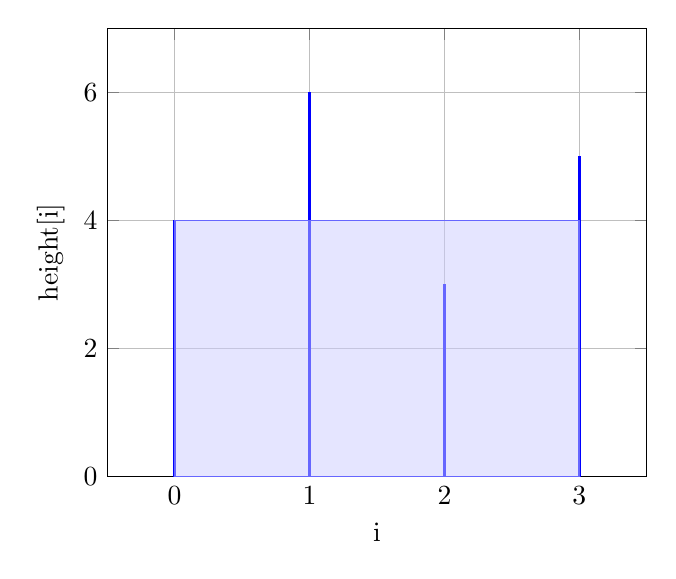
\begin{tikzpicture}
		\begin{axis}[
			xlabel={i},
			ylabel={height[i]},
			ymin=0, ymax=7,
			xmin=-0.5, xmax=3.5,
			xtick={0,1,2,3},
			grid=both,
			]
			% linee verticali per A = [4,6,3,5]
			\addplot[very thick, blue] coordinates {(0,0) (0,4)};
			\addplot[very thick, blue] coordinates {(1,0) (1,6)};
			\addplot[very thick, blue] coordinates {(2,0) (2,3)};
			\addplot[very thick, blue] coordinates {(3,0) (3,5)};
			
			% evidenzia il contenitore migliore tra i=0 e i=3
			\addplot[
			fill=blue!20,
			draw=blue!60,
			fill opacity=0.5 % 50% trasparente
			]
			coordinates {(0,0) (0,4) (3,4) (3,0) (0,0)};
		\end{axis}
	\end{tikzpicture}
	\caption{Container con area massima per $A = [4,6,3,5]$.}
\end{figure}

Il valore massimo è quindi
\[
\max_{0 \le i < j \le 3} \mathrm{area}(i,j) = 12,
\]
ottenuto per la coppia di indici $(i,j) = (0,3)$.

\begin{softnote}
	Nell'esempio: area$(0,3) = (3-0) \times \min(4,5) = 3 \times 4 = 12$ è la massima possibile.
\end{softnote}

Quindi il pseudocodice per questo problema computazionale è il seguente:

\begin{algorithm}[H]
	\caption{Container With Most Water}
	\label{alg:container-most-water}
	
	\KwIn{Array $height[0 \dots n-1]$ di interi non negativi}
	\KwOut{Massima area d'acqua contenibile}
	
	$left \gets 0$\tcp*{Puntatore sinistro}
	$right \gets n - 1$\tcp*{Puntatore destro}
	$maxArea \gets 0$\tcp*{Area massima trovata finora}
	
	\While{$left < right$}{
		$width \gets right - left$\tcp*{Larghezza del contenitore}
		$h \gets \min(height[left],\; height[right])$\tcp*{Altezza = lato più basso}
		$area \gets width \cdot h$\tcp*{Area del contenitore corrente}
		$maxArea \gets \max(maxArea,\; area)$\tcp*{Aggiorna massimo}
		
		\If{$height[left] < height[right]$}{
			$left \gets left + 1$\tcp*{Sposta il lato più basso verso il centro}
		}
		\Else{
			$right \gets right - 1$\tcp*{Sposta il lato più basso verso il centro}
		}
	}
	\Return{$maxArea$}\tcp*{Restituisce l'area massima}
\end{algorithm}

\begin{softnote}
	\textbf{Tecnica dei due puntatori:}
	
	\begin{enumerate}
		\item Partiamo dai due estremi dell'array (left=0, right=n-1)
		\item Calcoliamo l'area del contenitore corrente
		\item Spostiamo verso il centro il puntatore che punta alla barra \textbf{più bassa}
		\item Ripetiamo fino a quando i puntatori si incontrano
	\end{enumerate}
	
	\textbf{Perché muoviamo il lato più basso?} Se muovessimo il lato più alto, la larghezza diminuirebbe e l'altezza resterebbe limitata dal lato basso: l'area peggiorerebbe sicuramente. Muovendo il lato basso abbiamo la \textit{possibilità} di trovare un lato più alto che migliori l'area.
\end{softnote}

\textbf{Complessità.}
Ad ogni iterazione del ciclo \texttt{while} viene spostato
solo uno dei due puntatori, che possono muoversi ciascuno al più $n-1$ volte.
Pertanto il numero di iterazioni è al più $n-1$ e il costo è
\[
T(n) = c_1 + c_2 (n-1) = \Theta(n).
\]
Lo spazio aggiuntivo utilizzato è costante, quindi $S(n) = \Theta(1)$.

\begin{nota}
	Complessità $\Theta(n)$ significa che l'algoritmo è \textbf{lineare}: raddoppiando la dimensione dell'input, il tempo raddoppia. Molto meglio di $\Theta(n^2)$ dove raddoppiando l'input il tempo quadruplica!
\end{nota}

\pagebreak
\subsubsection*{Prefisso più lungo comune fra più sequenze}

\begin{softnote}
	Questo problema è utile per capire come elaborare stringhe. L'idea è trovare la parte iniziale condivisa da tutte le stringhe in input.
\end{softnote}

\begin{algorithm}[H]
	\caption{Prefisso comune più lungo}
	\label{alg:prefisso-comune}
	
	\KwIn{Array $S[1 \dots n]$ di stringhe}
	\KwOut{Prefisso più lungo comune a tutte le stringhe}
	
	\tcp{Assumo che le stringhe di $S$ siano tutte diverse da \texttt{null}}
	
	$p \gets S[1]$\tcp*{Prefisso corrente}
	
	\For{$i \gets 2$ \KwTo $n$}{
		$p \gets \text{PrefissoComune}(p, S[i])$\tcp*{Prefisso tra $p$ e $S[i]$}
		\If{$p =$ stringa vuota}{
			\Return{p}\tcp*{Nessun prefisso comune}
		}
	}
	
	\Return{$p$}\tcp*{Prefisso comune più lungo}
\end{algorithm}

\begin{softnote}
	\textbf{Come funziona?}
	
	\textbf{Esempio:} $S = [\text{``fiore''}, \text{``fiorire''}, \text{``fioraio''}]$
	\begin{enumerate}
		\item $p = \text{``fiore''}$ (prima stringa)
		\item PrefissoComune($\text{``fiore''}$, $\text{``fiorire''}$) = $\text{``fiori''}$
		\item PrefissoComune($\text{``fiori''}$, $\text{``fioraio''}$) = $\text{``fior''}$
		\item Risultato: $\text{``fior''}$
	\end{enumerate}
	
	L'idea è semplice: confrontiamo il prefisso corrente con ogni stringa successiva, accorciandolo se necessario.
\end{softnote}

\noindent\textbf{Invariante:} Dopo ogni iterazione del ciclo, $p$ è il prefisso comune più lungo delle prime $i$ stringhe.

\textbf{Complessità.}
Sia $n$ il numero di stringhe in $S$ e sia $m$ la lunghezza della
stringa più corta. Ad ogni passo del ciclo la funzione
\texttt{PrefissoComune} confronta al più $m$ caratteri, quindi
\[
T(n,m) = c_1 + c_2 (n-1)m = \Theta(nm).
\]
Lo spazio aggiuntivo utilizzato è costante, dunque $S(n,m) = \Theta(1)$.

\begin{nota}
	La complessità $\Theta(nm)$ significa che nel caso peggiore confrontiamo $m$ caratteri per ognuna delle $n$ stringhe. Se abbiamo 100 stringhe di 50 caratteri, facciamo al massimo $100 \times 50 = 5000$ confronti.
\end{nota}

\pagebreak
